\documentclass[usegeometry=true]{scrartcl}
\usepackage[ngerman]{babel}
\usepackage[T1]{fontenc}
\usepackage{lmodern}
\usepackage[utf8]{inputenc}
\usepackage{hyperref}
\usepackage{amssymb}
% Dimensionen bitte nicht ändern. 
\usepackage[left=2cm, right=2cm, top=2cm, bottom=2cm, bindingoffset=1cm, includeheadfoot]{geometry}
%Zeilenabstand bitte nicht ändern
\usepackage[onehalfspacing]{setspace}
\usepackage{graphicx}

\usepackage[backend=biber,style=numeric,]{biblatex}
\usepackage{csquotes}
\addbibresource{literatur.bib}

\begin{document}
% ----------------------------------------------------------------------------
\subject{Projektbericht zum Modul Information Retrieval und Visualisierung Sommersemester 2021}
\title{Visualisierung der Konflikte Afrikas\\ von 1997 bis 2021}
%\subtitle{Untertitel}% optional
\author{Marcus Gagelmann}% obligatorisch
%\date{10.9.2021}
\maketitle% verwendet die zuvor gemachte Angaben zur Gestaltung eines Titels
% ----------------------------------------------------------------------------
% Inhaltsverzeichnis:
%\tableofcontents
% ----------------------------------------------------------------------------
% Gliederung und Text:

\section*{Projekt}
Gitlab-Projekt:\\
\hspace*{10mm} \url{https://gitlab.informatik.uni-halle.de/apzvk/iruv_projekt}\\\\
Link zur Anwendung:\\
\hspace*{10mm} \url{https://users.informatik.uni-halle.de/~apzvk/index.html}\\\\
Letzter Programmcode-Commit:\\
\hspace*{10mm} c44327a (implementation notes, 2021-09-08)\\\\
Letzter Bericht-Commit:\\
\hspace*{10mm} 4ff7ba5 (Bericht: Rechtschreibkorrektur, 2021-09-11)\\

\section{Einleitung}
Afrika bildet mit einer Größe von mehr als 30 Millionen Quadratkilometern den zweitgrößten Kontinent der Erde. Insgesamt leben dort über 1,3 Milliarden Menschen, was etwa 17,2\% der Weltbevölkerung ausmacht. Wo jedoch Land und Menschen aufeinander treffen, dort sind auch Konflikte nicht weit entfernt. Seit vielen Jahren fällt Afrika solchen sowohl politischen als auch kriegerischen Auseinandersetzungen zum Opfer. Ursachen hierfür könnten die verbreitete Armut, misswirtschaftende Regierungen sowie die wertvollen Ressourcen des Kontinents sein, um nur einige mögliche Gründe zu nennen. Seit 1997 werden diese Konflikte durch das ACLED-Projekt dokumentiert. ACLED steht hierbei für \glqq Armed Conflict Location and Event Data\grqq{}. Die gesammelten Daten werden von ACLED auf ihrer Website \cite{acled} frei zugänglich zur Verfügung gestellt.\\

Nach nun beinahe 25 Jahren an Konfliktaufzeichnungen sind mittlerweile sehr große Datenmengen entstanden, welche einem außenstehenden Tabellenbetrachter kaum einen Überblick über das Gesamtgeschehen seit dem Aufzeichnungsbeginn geben können. Noch unwahrscheinlicher ist es, dass ein solcher Betrachter allein mithilfe der unaufbereiteten Daten Rückschlüsse auf mögliche Zusammenhänge zwischen den vielen Konflikten ziehen kann. Mit dieser Ausgangslage ist ein Verstehen der tatsächlichen Lage in Afrika anhand der Daten unmöglich. Hierdurch könnten mögliche Maßnahmen zur Verbesserung der Situation des Kontinents weniger effektiv ausfallen, als wenn das volle Potenzial der Daten ausgeschöpft werden würde.\\

Aus diesem Problem ergibt sich die Fragestellung, ob der gewählte Datensatz hilfreiche Aussagen zu Zusammenhängen ermöglicht, welche die Opfer der Konflikte der letzten 25 Jahre betreffen. Das Ziel dieser Arbeit ist deshalb die Bereitstellung einer Anwendung, welche eine Analyse der Todesopferanzahlen der Afrikakonflikte ermöglicht.

\subsection{Anwendungshintergrund}
Mithilfe der im Rahmen dieser Arbeit entwickelten Anwendung werden einzelne Konflikte für einen Gesamtüberblick über eine oder mehrere Regionen Afrikas zusammengefasst, sowie nach einzelnen Jahren sortiert und hierbei auch mehrdimensional visualisiert. Insgesamt umfasst das Programm zwei verschiedene Ansichten, welche jeweils eine Menge von Konflikten auf unterschiedliche Art und Weise darstellen. In der Hauptansicht, dem Scatterplot, ist es dem Nutzer möglich einen Überblick über die Konfliktdichte und die Opferzahlen zu unterschiedlichen Zeitpunkten seit Aufzeichnungsbeginn zu erhalten. Die Zweitansicht, welche sich der Technik paralleler Koordinaten bedient, zeigt immer eine Teilmenge der Konflikte der Hauptansicht in jeweils drei Dimensionen. Hier kann der Nutzer einen genaueren Einblick erhalten, in welchem Monat eines Jahres welche Art von Konflikt wie viele Todesopfer forderte. Die Basismenge an Konflikten, welche für die Visualisierungen verwendet wird, ergibt sich aus der Menge aller Konflikte des Datensatzes, welche mithilfe eines Regionenfilters gekürzt wird. Dieser Filter wird vom Nutzer über eine dritte Ansicht in Form eines interaktiven Baumes gesteuert. Hier können sowohl die Konflikte größerer Regionen als auch die Konflikte einzelner Länder Afrikas in die visualisierte Gesamtmenge aufgenommen werden.

\subsection{Zielgruppen}
Als Zielgruppe für die Visualisierungsanwendung kommen Personen infrage, welche einen Überblick über die Konflikt- und Todesopferdichte zu verschiedenen Zeitpunkten und in verschiedenen Regionen des afrikanischen Kontinents erlangen wollen, sowie einen genaueren Einblick in die Art der Konflikte benötigen. Das Programm ist für einen schnellen Einstieg und einen groben Überblick in der Thematik der Afrikakonflikte konzipiert. Aus diesem Grund benötigen Zielgruppen in der Regel kaum Vorwissen, um die Anwendung sinnvoll zu nutzen. Politisches und geografisches Vorwissen kann in manchen Anwendungsgebieten für das weitere Verständnis sinnvoll sein, ist aber keines Falls Voraussetzung um Erkenntnisse aus den Daten mithilfe der Anwendung zu gewinnen.\\

Die Verwendung einer solchen Anwendung ist bei Hilfsorganisationen zur Planung zukünftiger Einsätze denkbar. Hiermit könnten zukünftig diejenigen Regionen Afrikas ermittelt werden, welche langfristig die größten Opfer zu beklagen haben und aufbauend auf diesen Fakt weitere Hilfsleistungen am dringendsten benötigen. Weiterhin können Hilfskräfte leicht einen Eindruck von der Art der bisherigen Konflikte einer bestimmten Region bekommen und damit zukünftige Einsätze besser auf diese Art von Konflikten vorbereiten.\\

Ein weiteres Anwendungsgebiet könnte die Risikoeinschätzung für Reisen durch das Auswärtige Amt \cite{aa} darstellen. Hier bietet die Anwendung die Möglichkeit, die Gefahr für deutsche Reisende in Konfliktbelasteten Regionen Afrikas besser beurteilen zu können. Gäbe es in den letzten Jahren eine hohe Dichte an politischen Unruhen oder Todesopfer durch Kampfhandlungen, so können hierdurch Urlaubs- und Durchreisende rechtzeitig vor Gefahren gewarnt werden.

\subsection{Überblick und Beiträge}
Dieses Projekt setzt sich zusammen aus dem Datensatz des ACLED-Projekts von 1997 bis 2021 und drei unterschiedlichen Visualisierungstechniken, welche interaktiv miteinander verbunden wurden. Vom verwendete Datensatz werden insgesamt sechs Felder jedes Datenobjektes für die Umsetzung der Anwendung genutzt. Hierzu gehören das Jahr sowie das Datum des Konflikts, die Art des Konflikts, die Region sowie das Land in dem ein Konflikt vorgefallen ist und die Anzahl an Todesopfern, welche ein Konflikt forderte. Die in dem Programm verwendeten Visualisierungstechniken beschränken sich auf eine Hauptansicht mit einem Scatterplot und einer umschaltbaren Zweitansicht, welche parallele Koordinaten zur Umsetzung verwendet. Zusätzlich gibt es noch einen Regionenfilter, welcher mithilfe expliziter Bäume anschaulich umgesetzt wurde. Im Scatterplot findet weiterhin die sogenannte X-Ray-Technik Anwendung, welche dem Nutzer Überlagerungen von Punkten aufzeigen kann. \\

Die Beiträge dieses Projekts belaufen sich auf die Auswahl, die Verarbeitung sowie die Visualisierung von Daten der Konflikte in Afrika in den Jahren 1997 bis 2021. Ganz konkret wird hierbei der Prototyp einer möglichen Anwendung diskutiert, welcher dem Nutzer die gewählten Daten und deren Zusammenhänge als interaktiv verbundenes System näher bringen soll. Hierbei werden die einzelnen Teile der Anwendung kritisch betrachtet, gelungene Ansätze hervorgehoben und Vorschläge zur weiteren Verbesserung geäußert.

\section{Daten} \label{sec:daten}

\begin{figure}[]
\begin{center}

\begin{tabular}{lllll}
 \parbox{5.5cm}{
 \begin{enumerate}
  \item ISO
  \item EVENT\_ID\_CNTY
  \item EVENT\_ID\_NO\_CNTY
  \item EVENT\_DATE
  \item YEAR
  \item TIME\_PRECISION
  \item EVENT\_TYPE
  \item SUB\_EVENT\_TYPE
  \item ACTOR1
  \item ASSOC\_ACTOR\_1
 \end{enumerate}}
 &
 \parbox{4.5cm}{
 \begin{enumerate}
 \setcounter{enumi}{10}
  \item INTER1
  \item ACTOR2
  \item ASSOC\_ACTOR\_2
  \item INTER2
  \item INTERACTION
  \item REGION
  \item COUNTRY
  \item ADMIN1
  \item ADMIN2
  \item ADMIN3
 \end{enumerate}}
 &
 \parbox{5cm}{
 \begin{enumerate}
 \setcounter{enumi}{20}
  \item LOCATION
  \item LATITUDE
  \item LONGITUDE
  \item GEO\_PRECISION
  \item SOURCE
  \item SOURCE\_SCALE
  \item NOTES
  \item FATALITIES
  \item TIMESTAMP
 \end{enumerate}}

\end{tabular}

\caption{Dimensionen des ACLED-Datensatzes}
Quelle: Eigene Darstellung
\label{dimensions}
\end{center}
\end{figure}

Der Datensatz des ACLED-Projekts für die Afrikakonflikte von 1997 bis 2021 beinhaltet insgesamt 65443 einzelne Datenobjekte bzw. Datenzeilen, welche jeweils einen gesonderten Konflikt repräsentieren. Jedes Datenobjekt des Datensatzes liegt in insgesamt 29 Dimensionen vor, welche im Einzelnen in Abbildung \ref{dimensions} eingesehen werden können. Verwendet werden von diesen Dimensionen in der Anwendung EVENT\_DATE, YEAR, EVENT\_TYPE, REGION, COUNTRY und FATALITIES. Diese gewählten Dimensionen beinhalten alle für das Programm benötigten Daten und bieten den Vorteil, uncodiert und fast ausschließlich in direkt verwendbarer Form vorzuliegen. Direkt verwendbar bedeutet hierbei, dass die Dimensionen keine weitere Verarbeitung benötigen und direkt in einfache Elm-Datenstrukturen (Int und String) umgewandelt werden können. Lediglich die Dimension EVENT\_DATE bedarf einer zusätzlichen Übersetzerfunktion, welche genutzt werden kann, um den erhaltenen Event-Date-String auf den zugehörigen Monat zu mappen.\\

Es bleibt die Frage, inwieweit sich der Datensatz des ACLED-Projekts für die Zielgruppen dieser Arbeit eignet. Die eindeutigen Daten zu Zeitpunkt, Name des Landes und Todesopfern eignen sich gut für Hilfsorganisationen, um zu ermitteln, welche Länder aktuell am meisten unter den Konflikten leiden. Hierdurch kann eine Vorauswahl getroffen werden, welche Länder momentan Hilfsleistungen benötigen könnten. Mithilfe der Art des Events (EVENT\_TYPE) kann es diesen Organisationen weiterhin gut möglich gemacht werden, die Problemlage im Land besser zu verstehen und einen potenziellen Hilfseinsatz präziser auf eine bestimmte Art von Konflikten vorzubereiten. Bei der Aufgabe einer Gefahreneinschätzung für Reisende durch das Auswärtige Amt kann mithilfe der gewählten Dimensionen des Datensatzes durchaus auch geholfen werden. Informationen wie die Konfliktdichte, die Todesopferdichte und auch die Konfliktarten in einer bestimmten Region lassen eine erste Einschätzung zu der Situation eines Landes und zur Gefahr für Reisende zu.\\ Eine Verwendung der vorhandenen Geodaten zur Erweiterung der Anwendung durch eine interaktive Karte wäre durchaus denkbar und würde den Zielgruppen beim Verstehen von Zusammenhängen zwischen den Geodaten und den Konfliktdaten zusätzlich helfen. Eine solche Anwendung der Geodaten würde jedoch aufgrund von Problemen bei der Datenaufbereitung sowie der nötigen Ergänzung des Projektes durch Polygondaten für Länderumrisse den Rahmen dieser Arbeit sprengen.\\ Es ist an dieser Stelle wichtig anzumerken, dass die Daten, welche im Programm Anwendung finden, nicht allein ausreichen, um die genannten Aufgaben der Zielgruppen zu erfüllen. Da sowohl die Planung von Hilfseinsätzen, als auch die Einschätzung von Gefahrenländern Auswirkungen auf die Sicherheit von Menschenleben haben kann, ist eine Ergänzung des Datensatzes durch zusätzliche detaillierte Informationen zur Politik, Mentalität, Religion und anderen landes- und regionsspezifischen Informationen abseits der aufgezeichneten Konflikte unabdingbar. Beispielsweise kann offen gezeigte Homosexualität momentan in der Republik Kongo zu willkürlichen Verhaftungen wegen angeblich sittenwidrigen Verhaltens führen \cite{aa-kongo}, was unbedingt bei einer Gefahreneinschätzung des Landes für westliche Reisende berücksichtigt werden sollte. Diese Information könnte jedoch nicht aus dem gewählten Datensatz ermittelt werden, da sich dieser lediglich auf größere Konflikte und nicht auf einzelne Verhaftungen innerhalb der Republik Kongo stützt.

\subsection{Technische Bereitstellung der Daten}

Bereitgestellt werden die verwendeten Daten von Kaggle \cite{kaggle}, einer Plattform, auf der unter anderem Datensätze für Data-Science-Projekte geteilt werden können. Eine andere Möglichkeit für den Download der Daten bietet die Seite des ACLED-Projekts \cite{acled}. In dieser Arbeit wird der Datensatz von Kaggle verwendet, da die dort bereitgestellten Daten, anders als auf der ACLED-Seite, bereits nach Konflikten im Raum Afrika gefiltert sind. Läd man den Datensatz direkt von Kaggle herunter, so erhält man diesen im CSV-Dateiformat. Als Separator werden hierbei Semikolons verwendet. Die Größe des Datensatzes beläuft sich auf etwa 30,5 MB (30.565.061 Bytes) im Standard CSV-Format, welche sich jedoch auf 62,4 MB (65.467.818 Bytes) mehr als verdoppelt nach einer Umwandlung der Daten in ein JSON-Dateiformat. Die Notwendigkeit für eine solche Umwandlung des Formats wird im Kapitel \ref{sec:datenvorverarbeitung} genauer besprochen.\\ Jede Dimension des Datensatzes ist grundsätzlich entweder als Integer-Wert (Ziffern ohne Komma oder Anführungszeichen) oder als String-Wert (Zeichenfolgen in Anführungszeichen) gegeben. Hierzu gehören auch die Werte LATITUDE und LONGITUDE, welche eigentlich Float-Werte darstellen sollten. Dies stellt ein Problem, welches vor der eigentlichen Verwendung der Daten beim Einlesen durch eine Aufbereitung behoben werden müsste. Die Angaben in LATITUDE und LONGITUDE liegen als String vor, welcher unterschiedlich lange Ziffernfolgen enthalten kann. Hierbei ist keine Kommastelle angegeben, wodurch die Koordinaten des Konflikts nicht eindeutig wiedergegeben werden. Beispielsweise existiert ein Konflikt mit dem Breitengrad 36672 und dem Längengrad 2789. Mit diesen Daten könnten die Koordinaten (3.6672, 27.89) gemeint sein, welche eine Position im Wald in der Demokratischen Republik Kongo bestimmen. Aufgrund der Größe des Kontinents könnten hier jedoch auch die Koordinaten (36.672, 2.789) infrage kommen, welche eine Position in der Stadt Koléa in Algerien beschreiben. In diesem Fall ist die zweite Möglichkeit korrekt. Es wird jedoch ersichtlich, dass die Position des Kommas in den Breiten- und Längengraden nicht trivial bestimmt werden kann. Einige weitere Dimensionen des Datensatzes sind ebenfalls nicht sehr leicht zugänglich. Die Dimension INTERACTION liegt beispielsweise, neben einigen anderen, nur als numerischer Code vor. Um die tatsächliche Art der Interaktion der betroffenen Parteien ermitteln zu können, müsste hierfür vorher ein Übersetzer mithilfe des Codebooks des ACLED-Projekts \cite{acled-codebook} gebaut werden.\\ Das Feld EVENT\_DATE, welches tatsächlich im Programm verwendet wird, besitzt ebenfalls eine erwähnenswerte Formatierung. Die Datumsangaben liegen nämlich im Format \glqq TT-MMMMM-JJJJ\grqq{} vor, wobei der Monat in französischer Sprache ausgeschrieben wird. Hier werden an späterer Stelle (siehe Kapitel \ref{sec:datenvorverarbeitung}) weitere Datenverarbeitung nötig sein. Zuletzt bietet der gewählte Datensatz noch Metadaten, welche sich in die ungekennzeichnet in die anderen Datenfelder einordnen. Hierzu gehören die Dimensionen wie TIME\_PRECISION, welche einen Code für die Genauigkeit der Zeitangaben dieses Datenobjektes angibt und GEO\_PRECISION, welche einen Code für die Genauigkeit der Positionsangaben dieses Datenobjektes angibt. Auch diese müssten bei Bedarf mithilfe eines Übersetzers ausgelesen werden und anschließend zur Umwandlung einer Position/eines Zeitpunktes in einen Bereich/einen Zeitraum verwendet werden.\\

\subsection{Datenvorverarbeitung} \label{sec:datenvorverarbeitung}
Im Rahmen dieses Projektes wurde die Entscheidung getroffen, den vorliegenden CSV-Datensatz in ein entsprechendes JSON-Dateiformat umzuwandeln. Zum einen bietet das JSON-Dateiformat den Vorteil für den Menschen besser lesbar zu sein, was sich als Hilfe bei manuellen Auswertungen während der Entwicklung des Programms herausstellte. Weiterhin werden bei der Konvertierung in das JSON-Format Objektstrukturen erstellt und im Datensatz gespeichert, welche von Elm beim Einlesen der Daten direkt in Records übersetzt werden können. Würde der Datensatz als CSV eingelesen werden, so müsste Elm zuerst die gesamte Datei als Zeichenkette einlesen und diese anschließend, aufgrund der fehlenden Objektstrukturen, aufwändiger während der Laufzeit parsen.\\ Beim Start des Programms müssen initiale Datenvorverarbeitungsschritte durchgeführt werden, um den View-Funktionen alle nötigen Daten zur korrekten Visualisierung bereitstellen zu können. Hierzu gehört eine initiale Filterung der Regionen und Länder, um eine hilfreiche Startansicht gewährleisten zu können. Für diese Startansicht werden alle Konflikte herangezogen, welche sich seit 1997 im Land Ghana zugetragen haben. Hierfür wird die Funktion filterConflicts verwendet, welcher eine Liste aller Konflikte sowie alle aktiv geschalteten Länder und Regionen übergeben werden. Anschließend wird mithilfe der aktiven Länder und Regionen eine Liste derjenigen Länder erstellt, welche letztendlich angezeigt werden sollen. Dies ist wichtig, da in diesem Schritt auch die Länder ganzer aktiver Regionen zur ursprünglichen Liste aktiver Länder hinzukommen können. Letztendlich wird mithilfe der resultierenden Liste aktiver Länder die Liste aller Konflikte gefiltert. Hierbei werden alle Konflikte beibehalten, dessen Ländername mit einem Land aus der Liste aktiver Länder übereinstimmt.\\ Zusätzlich zur initialen geografischen Filterung müssen auch die französischen Datumsangaben der Dimension EVENT\_DATE mit Tag, Monat und Jahr in die benötigten englische Monatsangaben übersetzt werden. Eine Übersetzung in ein auf den Tag genaues Datum wäre an dieser Stelle ebenfalls denkbar. Monatsangaben reichen hierbei jedoch von der Präzision her aus, um den Überblick innerhalb der parallelen Koordinaten zu bewahren. Da die Dimension EVENT\_DATE als String gegeben wird und die französischen Monatsnamen nicht variieren, reicht hier eine einfach Übersetzerfunktion aus, welche einen EVENT\_DATE-String auf die französischen Monatsnamen durchsucht und den zugehörigen englischen Monatsnamen zurückgibt. Mithilfe dieser Funktion kann anschließend eine Liste aller EVENT\_DATE-Strings für die weitere Verwendung zu einer Liste mit englischen Monatsbezeichnungen gemappt werden.\\ Für die Visualisierung aller Konflikte eines einzelnen Jahres in der Zweitansicht als parallele Koordinaten wurde unter anderem die EVENT\_TYPE-Dimension in der Anwendung dieses Projektes herangezogen. Hier wurde jedoch bewusst darauf verzichtet die untergeordnete SUB\_EVENT\_TYPE-Dimension ebenfalls zu visualisieren. Durch die Verwendung dieser Dimension würde die Zweitansicht des Programms zwar theoretisch einen höheren Detailgrad an Informationen zu den konkreten Geschehnissen eines Konflikts vermitteln. Es existieren jedoch 23 verschiedene Ausprägungen der SUB\_EVENT\_TYPE-Dimension, wodurch ein Nutzer bei Verwendung dieser Dimension leicht den Überblick verlieren könnte. Da jede einzelne Ausprägung dieser Dimension als relativ lange Zeichenkette in die Visualisierung eingebracht werden müsste, könnten sogar Überlagerungen der Achsenbeschriftungen auftreten. Eine Reduktion des Darstellungsaufwands ist an dieser Stelle keine Möglichkeit, weil jede einzelne Ausprägung der SUB\_EVENT\_TYPE-Dimension eine recht komplexe Information vermittelt, welche nur schwer abgekürzt werden kann. Ein Beispiel hierfür ist ein SUB\_EVENT\_TYPE des EVENT\_TYPE \glqq Battles\grqq{}, welcher mit \glqq Non-state actor overtakes territory\grqq{} bezeichnet wird.\\

\section{Visualisierungen}
\subsection{Analyse der Anwendungsaufgaben}

Insgesamt werden im Rahmen dieser Arbeit zwei Anwendungsaufgaben betrachtet. Zuerst soll die Anwendung Hilfskräften, welche zukünftige Einsätze in Afrika planen, einen schnellen aber gut verständlichen Überblick über die betroffensten Länder aktueller Konflikte verschaffen. Zusätzlich sollte es Mitarbeitern von Behörden wie dem Auswärtigen Amt mithilfe des Programms möglich sein, die Gefahrenlage für Reisende der westlichen Welt einschätzen zu können.\\

Für die erste Aufgabe ist es wichtig, dass die Zielgruppe gezielt Regionen und Länder auf die zugehörige Todesopferdichte untersuchen kann. Weiterhin sollten die Nutzer des Programms in der Lage sein, die am häufigsten vorkommenden Konfliktarten prüfen zu können. Diese Informationen sind nötig, um eingrenzen zu können, welche Regionen und Länder zusätzliche Hilfeleistungen am dringendsten benötigen. Weiterhin ist es nötig, die durchschnittliche Anzahl an Todesopfern bei einem Konflikt eines bestimmten Landes oder einer Region einschätzen zu können, um die Quantität der zukünftigen Hilfseinsätze festzulegen. Zuletzt ist ein Überblick über die häufigsten Konfliktarten notwendig, damit Hilfsorganisationen einschätzen können, ob und wie viele Sicherheitskräfte einen eventuellen Hilfseinsatz begleiten müssen.\\ Die nötigen genannten Informationen können zum Teil aus der Anwendung gewonnen werden. Beispielsweise hilft der Scatterplot in Verbindung mit dem Regionenfilter beim Aufbau eines mentalen Modells zur Todesopferdichte der verschiedenen Regionen in den letzten Jahren. Hierbei verinnerlicht der Nutzer einen Eindruck von denjenigen Jahren, in denen sich besonders viele Konflikte überlagern, sowie einzelnen \glqq ausreißenden\grqq{} Konflikten, welche eine besonders hohe Anzahl an Todesopfern forderten. Mithilfe von Parallelen Koordinaten können anschließend einzelne Jahre noch präziser betrachtet werden, um den ersten Überblick über die Opfer dieses Jahres zu festigen und grob einschätzen zu können, welche Art von Konflikten die meisten Opfer forderte.\\ Kritisch betrachtet werden sollte die Fähigkeit der Anwendung, die durchschnittliche Todesopferanzahl eines Jahres zu vermitteln. Mithilfe der verwendeten X-Ray-Technik des Scatterplots sind zwar Konflikthäufungen auszumachen, eine genaue Einschätzung des Todesopferdurchschnitts ist jedoch durch die Verwendung absoluter Zahlen und Überlagerungen nur bedingt möglich. Hier sollte entweder die Anwendung mithilfe weitere Ansichten ausgebaut, oder externe Quellen zur Ergänzung des Programms herangezogen werden. Nicht nötig sind für diese Anwendungsaufgabe die Jahre, welche sich bereits weit in der Vergangenheit befinden. Hier können keine Informationen abgelesen werden, welche aktuelle Hilfseinsätze beeinflussen würden.\\

Für die Aufgabe der Gefahreneinschätzung durch das Auswärtige Amt, welche die Anwendung unterstützen soll, wird ein ähnliches mentales Modell wie für die erste Anwendungsaufgabe benötigt. Hier ist ein breiter Überblick über die Konfliktdichte eines Landes in den letzten Jahren wichtig, um effizient Kandidaten unter den Ländern auszumachen, welche anschließend gründlich auf eine potenzielle Einreisewarnung untersucht werden müssen. Für diese Anwendungsaufgabe könnten weit vergangene Jahre ebenfalls interessant sein, um die Konfliktgeschichte eines Landes besser nachempfinden zu können und damit das zukünftige Gefahrenpotenzial besser einschätzen zu können.\\

\subsection{Anforderungen an die Visualisierungen}
Im Rahmen dieser Arbeit soll eine Anwendung entstehen, welche eine unterstützenden Rolle bei Analysen der Afrikakonflikte von 1997 bis 2021 einnimmt. Die Hauptanforderung an das Programm ist hierfür, dem Nutzer einen schnellen aber effektiven Überblick darüber zu geben, welche Regionen Afrikas besonders von Konflikten geprägt sind und welche Todeszahlen sich hieraus im Vergleich zu anderen Regionen ergeben. Zu diesem Zweck sollten die unterschiedlichen Visualisierungsansichten des Programms in einem relativ \glqq leichten\grqq{} Design gehalten werden. Eine Überzahl an gleichzeitig gezeigten Informationen könnte zwar den Detailgrad der Anwendung erhöhen, der eigentliche Sinn der Anwendung würde hierdurch jedoch in den Hintergrund gerückt werden.\\ Die Filterfunktion für Regionen und Länder ist einer der wichtigsten Teile der Anwendung und bedarf besonderer Sorgfalt bei der Entwicklung. Dem Nutzer muss es möglich sein, flexibel einzelne Länder und ganze Regionen Afrikas zum Filter für die anderen Visualisierungen hinzuzufügen. Zusätzlich sollten Nutzer der Anwendung jeder Zeit Feedback dazu bekommen, welche Konflikte aus welchen Ländern und Regionen ihm momentan angezeigt werden. Zuletzt ist es für den Nutzer durchaus sinnvoll, permanent die geografischen Zusammenhänge zwischen den filterbaren Ländern und Regionen vermittelt zu bekommen, um einen besseren Überblick über aktuelle Filtereinstellungen und deren Bedeutung zu bewahren.\\ Die Hauptaufgabe der Anwendung ist die Vermittlung eines Eindrucks der Schwere von Konflikten in verschiedenen Ländern und Regionen. Zu diesem Zweck sollte unbedingt eine Darstellung der Opferzahlen in Relation zu unterschiedlichen sinnvollen Dimensionsausprägungen erfolgen, um einzelne Ereignisse, ganze Länder und länderübergreifende Regionen zu einem bestimmten Zeitpunkt besser zu verstehen. Hierfür bieten sich beispielsweise Zeiteinheiten, Konfliktarten oder auch Geodaten an. Die Verwendung der Jahresdaten ist in diesem Fall besonders entscheidend für die Zielgruppen, um aktuelle Ereignisse von weit vergangenen unterscheiden zu können. Die genauere Untersuchung einzelner Jahre als \glqq visualisierter Ausschnitt\grqq{} könnte hierbei von Vorteil sein.\\

\subsection{Präsentation der Visualisierungen}
\subsubsection{Visualisierung Eins}

\begin{figure}[]
\begin{center}
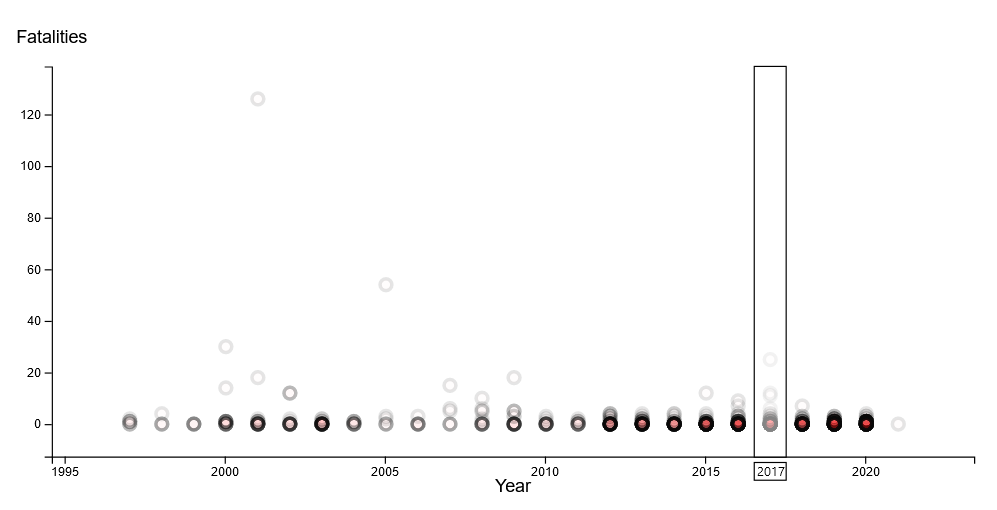
\includegraphics[width=12cm,height=10cm,keepaspectratio]{Scatterplot.PNG}%
\caption{Screenshot eines möglichen Scatterplots}
Quelle: Eigene Darstellung
\label{scatterplot}
\end{center}
\end{figure}

Die erste Visualisierung innerhalb der Anwendung ist beispielhaft in Abbildung \ref{scatterplot} zu sehen und zeigt einen zweidimensionaler Scatterplot, welcher sowohl die Dimension der Todesopferzahlen als auch die zugehörigen Jahre darstellt. Hierbei werden die Achsen dynamisch an die aktuell angezeigten Daten angepasst, um diese immer maximal auf die zur Verfügung stehende Fläche zu verteilen. Jeder Datenpunkt in der Visualisierung stellt einen Konflikt des ACLED-Datensatzes dar. Diese werden in der Darstellung mit einer hohen Transparenz angezeigt, um einen X-Ray-Effekt zu erzeugen, wodurch Überlappungen leicht erkannt werden können. Das Design der Datenpunkte ist geprägt durch einen dicken schwarzer Ring mit einer hohen Transparenz (alpha-Wert von 0.1), welcher mit einem Rotton gefüllt ist, der nochmal um ein zehnfaches transparenter ist (alpha-Wert von 0.01).\\ Das letzte Detail der Scatterplot-Visualisierung ist das interaktive Feature der Jahresauswahl. Hierfür wird der Scatterplot in gedachte Spalten eingeteilt, welche an Jahresachse ausgerichtet sind. Durch einen Hover der Maus über eine dieser Spalten erscheint für die Dauer des Hovers ein spaltenumfassendes Rechteck mit schwarzen Rändern und stark transparenter weißer Füllung. Zusätzlich erscheint auf der Jahresachse das betreffende, schwarz umrandete Jahr für die Dauer des Maus-Hovers. Ein Klick auf eine der markierten Flächen lässt die Anwendung in die zweite Visualisierung (siehe Abbildung \ref{parallelCoordinates}) des ausgewählten Jahres wechseln.\\ Die Anforderung an die Visualisierung, einen ersten schnellen Überblick über die Todesopferzahlen der angezeigten Regionen zu gewähren, wird von der ersten Ansicht größtenteils erfüllt. Grund hierfür ist das minimalistische aber leicht verständliche Design, welches auf der allgemein bekannten Visualisierungstechnik des zweidimensionalen Scatterplots beruht. Dieser Fakt in Kombination mit nur zwei unterschiedlichen verwendeten Farben ermöglicht es einem Betrachter, ohne längere Betrachtungszeit einen Überblick über die präsentierten Informationen zu gewinnen. Der Gehalt der präsentierten Informationen könnte wiederum noch höher sein.\\ Ein Problem der ersten Visualisierung ist die Umsetzung der X-Ray-Technik. Diese vermittelt zwar eindeutig und auf den ersten Blick höhere und weniger hohe Konfliktdichten, wie viele Datenpunkte in solchen Clustern jedoch genau vorhanden sind, kann der Betrachter nur schlecht erahnen. Ab einer gewissen Konfliktüberlappung gleichen sich die Cluster zu stark um sie präzise unterscheiden zu können. Dies könnte seinen Ursprung darin haben, dass ein linearer Anstieg des Helligkeitsstimulus nur zu einem sublinearen Zuwachs an wahrgenommener Helligkeit (oder Dunkelheit) korrespondiert (siehe Vorlesungsskript Seite 117). In anderen Worten bedeutet das, dass ab einer gewissen Sättigungs- bzw. \glqq Dunkelheitsstufe\grqq{} bei einem Datenpunkte bei gleich bleibender, linearer Verdunklung immer geringere Veränderung für das menschliche Auge wahrnehmbar ist. Hier könnte die Anwendung einer Gammakorrektur Abhilfe verschaffen, welche die linearen Helligkeitsabstufungen auf eine andere gewünschte Weise skalieren kann. Hiermit könnten auch bei höheren Datenpunktdichten noch wahrnehmbare Unterschiede herbeigeführt werden.\\ Ein weiteres Problem des Scatterplots ist die Verteilung der Datenpunkte auf der Fatalities-Achse. Hier ist bei fast allen möglichen Regionszusammensetzungen zu beobachten, dass sich der Großteil der Datenpunkte im untersten Bereich der Grafik ansammeln. Einzelne Ausreißer lassen den Wertebereich der Fatalities-Achse jedoch bis zu weit überdurchschnittlichen Werten verlaufen. Um die Datenpunkte auf dieser Grundlage besser in der Grafik zu verteilen, könnte hier eine logarithmische statt einer linearen Skalierung der Fatalities-Achse angebracht sein. Hierdurch würden die stark komprimierten Datenpunkte am unteren Ende der Grafik eventuell besser im oberen Bereich verteilt werden. Hierdurch würde zum einen der Platz innerhalb der Grafik besser zur Informationsdarstellung genutzt werden, zum anderen könnte dieser Ansatz ebenfalls beim ersten Problem der zu hohen Datenpunktdichte helfen.\\

\subsubsection{Visualisierung Zwei}

\begin{figure}[]
\begin{center}
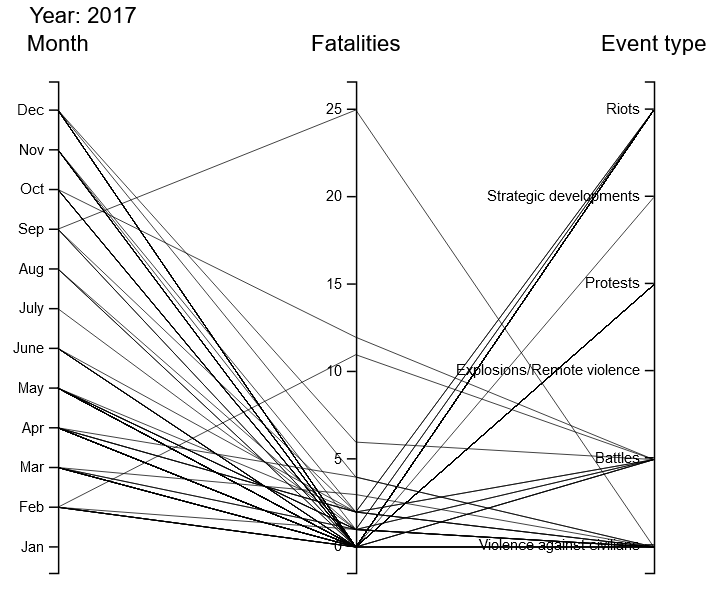
\includegraphics[width=12cm,height=10cm,keepaspectratio]{ParalleleKoordinaten.PNG}%
\caption{Screenshot einer möglichen Darstellung paralleler Koordinaten}
Quelle: Eigene Darstellung
\label{parallelCoordinates}
\end{center}
\end{figure}

Die zweite Visualisierung des Projektes zeigt einige Dimensionen von Konflikten aus ausgewählten Regionen, dargestellt als parallele Koordinaten. Zu diesem Zweck wurden drei parallele Achsen angelegt, eine für jede Datendimension, wie in Abbildung \ref{parallelCoordinates} zu sehen ist. Auf die erste dieser Achsen wird die Dimension EVENT\_DATE einzelner Konflikte abgebildet, welche in der Datenvorverarbeitung (siehe Kapitel \ref{sec:datenvorverarbeitung}) bereits auf den Monat, in welchem das Ereignis stattgefunden hat, reduziert wurde. Die anderen beiden Achsen beschreiben, ohne weitere Datenaufbereitung, die Anzahl der Todesopfer bei einem Konflikt (FATALITIES) und die Art eines Konflikts (EVENT\_TYPE). Einzelne Konflikte werden in dieser Visualisierung als dünne schwarze Pfade dargestellt. Diese verlaufen von ihrem zugehörigen Monat auf der linken Seite über ihr zugehörige Todesopferanzahl in der Mitte bis hin zu ihrer zugehörigen Konfliktart auf der rechten Seite. Das aktuell eingestellte Jahr für diese Visualisierung ist in der oberen linken Ecke zu erkennen.\\ Aufgrund der höheren Anzahl an Datendimensionen, welche sich größtenteils von denen der ersten Visualisierung unterscheiden, besitzt diese Darstellung einen höheren und anderen Informationsgehalt im Vergleich zur ersten. Trotzdem ist die verwendete Anzahl an Dimensionen mit lediglich dreien immer noch relativ gering. Zum einen trägt dies zu dem Anwendungsziel bei, die Visualisierungen für das schnelle Verstehen durch den Nutzer zu designen. Eine insgesamt recht geringe Dimensionsvielfalt zusammen mit der Verwendung von nur einer Farbe und einer oft nur geringen Anzahl an visualisierten Konflikten sorgt in dieser Darstellung beim Nutzer für einen schnellen Überblick, um effizient mehrere Versionen der zweiten Visualisierung zu verstehen. Es ist jedoch zu beachten, dass aufgrund dieses Minimalismus Potenzial verloren geht, dem Nutzer Informationen in größerer Qualität und Quantität zu vermitteln. Mithilfe der Achse der Dimension EVENT\_DATE hätte beispielsweise auch das gesamte Jahr in Tagesabstufungen und nicht in Monatsabstufungen abgebildet werden können. Außerdem gibt es durchaus weitere interessante Dimensionen (SUB\_EVENT\_TYPE, ACTOR1, ACTOR2, etc.), welche man zusammen mit den dargestellten Daten in Bezug hätte setzten können. Die verwendeten Dimensionen der zweiten Visualisierung wurden ausgewählt, um ein besseres Verständnis beim Nutzer zu schaffen für den Zeitpunkt und die Umstände, welche zu der zugehörigen Anzahl an Todesopfern während eines Konfliktes führten. Die FATALITIES-Achse wurde in der Mitte platziert, um zu beiden anderen Dimensionen in direkter Relation zu stehen und eine räumliche Nähe zu den anderen Achsen zu schaffen.\\ Die zweite Visualisierung erfüllt die Aufgabe, dem Nutzer einen genaueren Ausschnitt aus der Menge aller Konflikte der gewählten Region zu beschreiben. Hierfür wird das sogenannte \glqq Slicing\grqq{} verwendet, welches eine Methode der Datenanalyse darstellt. Dabei wird aus einem Datenwürfel eine Scheibe \glqq herausgeschnitten\grqq. In diesem Fall wird ganz konkret die Dimension YEAR der ersten Visualisierung auf ein einzelnes Jahr eingeschränkt, was gut in Abbildung \ref{scatterplot} durch die zugehörige Hover-Visualisierung verdeutlicht wird.\\ Ein Nachteil dieser Visualisierung ist, ähnlich wie schon beim Scatterplot, dass die Untersuchung einzelner Konflikte hier nur in Ausnahmefällen möglich ist. Oft ist nicht genau erkennbar, wie viele Konflikte sich auf einer Linie überlagern. Bei Betrachtung der gesamten Abbildung wird aber durchaus deutlich, in welchen Ausprägungen der verschiedenen Dimensionen hohe oder niedrige Konfliktdichten vorliegen. In Abbildung \ref{parallelCoordinates} ist beispielsweise zu sehen, dass hier die meisten Konflikte ungefähr gleich auf die Monate verteilt liegen, die meisten Konflikte weniger als fünf Todesopfer forderten und kein einziger Konflikt der Art \glqq Explosions/Remote violence\grqq{} war. Das Anwendungsziel des Gesamtüberblicks bleibt also durchaus erhalten. Um einen besseren Überblick über einzelne Konflikte zu behalten, könnten in dieser Visualisierung verschiedene Farben für verschiedene Konfliktarten oder aber auch, wie schon oben genannt, präzisere Skalen helfen, welche weniger Konfliktpfade auf ein und derselben Linie entstehen lassen würden.\\

\subsubsection{Visualisierung Drei}

\begin{figure}[]
\begin{center}
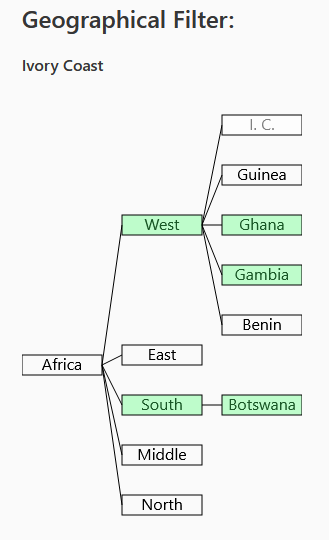
\includegraphics[width=12cm,height=10cm,keepaspectratio]{FilterTree.PNG}%
\caption{Screenshot eines möglichen Filterbaumes mit Maus-Hover über dem \glqq I. C.\grqq-Knoten}
Quelle: Eigene Darstellung
\label{filtertree}
\end{center}
\end{figure}

Die dritte und letzte Visualisierung liegt in der Form eines Baumes vor, wie in Abbildung \ref{filtertree} zu erkennen ist. Dieser Baum soll die verschiedenen, von Konflikten betroffenen Regionen Afrikas und deren geografisch-hierarchische Strukturen verdeutlichen. Die Knoten des Baumes bestehen aus Rechtecken mit schwarzem Rand und weißem Hintergrund, auf welchen der Name der zugehörigen Region zentral geschrieben steht. Verbunden sind diese Knoten durch schwarze Linien, welche die Kanten des Baumes repräsentieren. Der Baum ist in drei Ebenen eingeteilt, welche es als Nutzer zu verstehen gilt. Diese sind von links nach rechts vertikal ausgerichtet und beginnen in der ersten Ebene mit lediglich der Wurzel, welche das Wort \glqq Afrika\grqq{} enthält. Von diesem Afrikaknoten zweigen immer fünf Kanten nach rechts in die zweite Ebene ab und enden in Knoten, welche verschiedene Region Afrikas repräsentieren. Zuletzt kann auch noch jeder Regionsknoten in die dritte Ebene nach rechts ausgeklappt werden, um Knoten der verschiedenen konfliktbetroffenen Länder der zugehörigen Region zu zeigen. Hierüber bietet die Visualisierung interaktive Funktionen zur Filterung der in den anderen Darstellungen präsentierten Konflikte nach Regionen und Ländern an. Aktiv geschaltete Knoten werden hierbei grün von der ansonsten schwarz-weißen Darstellung hervorgehoben. Genaueres hierzu wird im Kapitel \ref{interaktion} beschrieben.\\ Auch diese Visualisierung ermöglicht dem Nutzer effizient an einen Überblick über die dargestellte Information zu gelangen, diesmal durch eine geringe Baumbreite und -tiefe, ein minimalistisches Komponentendesign mit wenigen unterschiedlichen Formen und Farben sowie ausklappbaren Teilbäumen, welche die Informationsflut auf den Nutzer so gering wie möglich halten.\\ Ursprünglich war für die Filterfunktion der Anwendung eine Liste von Checkboxen angedacht, welche sich jedoch als problematisch erwies. Bei 18 darzustellenden Ländern entstand eine zu lange Liste, um schnell gesuchte Länder finden zu können. Hierzu kommt die Tatsache, dass auf diese Weise zusätzlich keine gute Filterfunktion für gesamte Regionen existierte. Um dies zu ermögliche hätte die Liste von Checkboxen unter Umständen noch länger werden müssen und noch weniger Überblick geboten. Es ist also zu erkennen, dass die gewählte Möglichkeit einen hierarchischen Filter mithilfe eines Baumes zu realisieren und zu visualisieren durchaus Vorteile in diesem Anwendungsfall mit sich bringt.\\ Es besteht jedoch weiterhin auch ein Nachteil im Zusammenhang mit längeren Regions- und Ländernamen. Diese werden zum Teil zu lang um sie in einen Knoten einer Ebene zu schreiben. Für dieses Problem bieten sich verschiedene Lösungsansätze. Unter anderem wäre es denkbar, die Knotenhöhe zu vergrößern und lange Namen zweizeilig zu schreiben.\\ Eine andere Möglichkeit wäre es, den Baum und die Knoten weiter in die Breite zu vergrößern und somit die Namen einzeilig ausschreiben zu können. Beide Möglichkeiten nehmen jedoch zu viel Platz der Gesamtanwendung in Anspruch, wodurch der Filterbaum auf eine eigene Seite oder zumindest in ein eigenes Modal verlegt werden müsste. Hierdurch wäre es dem Nutzer jedoch nicht mehr möglich zu jedem Zeitpunkt die aktuellen Filtereinstellungen sowie die Regions- und Länderhierarchie einsehen zu können, wodurch wichtige Informationen beim Verstehen der anderen Visualisierungen verloren gehen. Da dieser Ansatz offensichtlich gegen das Anwendungsziel der Übersichtlichkeit arbeitet, wurde das Problem auf anderem Weg umgangen.\\ Die zu langen Namen in den Knoten des Baumes werden im Programm durch eine Elm-Funktion automatisch auf ihre Anfangsbuchstaben reduziert (z.B. \glqq I. C.\grqq{} für Ivory Coast). Beim Verstehen dieser Abkürzungen wird der Nutzer durch eine Maus-Hover-Funktion unterstützt, welche den vollen Namen eines Knotens oberhalb des gesamten Baumes anzeigt.\\

\subsection{Interaktion} \label{interaktion}
Die Interaktionsmöglichkeiten des Scatterplots beschränken sich auf die Möglichkeit der Spaltenauswahl, welche einen Ansichtswechsel zur zweiten Visualisierung, den parallelen Koordinaten, zur Folge hat. Hierbei wählt der Nutzer ein konkretes Jahr im Scatterplot aus, welches anschließend in der zweiten Visualisierung verwendet wird. Die Spaltenauswahl erfolgt durch das Hovern der Maus über einer Jahresspalte, wobei hier optisches Feedback gegeben wird (siehe Abbildung \ref{scatterplot}), und einem anschließendem Klick.\\ Die Visualisierung der parallelen Koordinaten beinhaltet zwei unterschiedliche Interaktionsmöglichkeiten. Zuerst existiert ein \glqq Back\grqq-Button, welcher einen Wechsel zurück zur Hauptansicht (Scatterplot) herbeiführt. Außerdem befinden sich daneben die Buttons \glqq Previous Year\grqq{} und \glqq Next Year\grqq. Diese können verwendet werden, um das im Scatterplot ausgewählte Jahr zu verringern oder zu erhöhen. Die Begrenzungen, an denen die entsprechenden Buttons deaktiviert werden, liegen bei den Jahren 1997 und 2021.\\ Zuletzt besitzt auch die Baumvisualisierung des Projektes Interaktionsmöglichkeiten in Form von aktivierbaren und deaktivierbaren Baumknoten. Aktive Knoten werden hierbei grün gekennzeichnet. Ein solches Umschalten eines Knotens erfolgt durch einen Maus-Hover über diesen, wobei ein optisches Feedback ausgelöst wird (siehe Abbildung \ref{filtertree}), gefolgt von einem Klick. In der Baumvisualisierung existieren Regionsknoten und Länderknoten. Wird ein Regionsknoten aktiv geschaltet, so werden alle seine Kinder, also die beinhalteten Länder der Region, \glqq ausgeklappt\grqq. Wird unter diesen Länderknoten nun keiner aktiv geschaltet, so werden die Datenpunkte der ganzen Region mit allen inbegriffenen Ländern angezeigt. Wird dieser Zustand nun durch die Auswahl einzelner Länder unterhalb des aktiven Regionsknotens verändert, so werden nur noch die aktiven Länder des aktiven Regionsknotens visualisiert. In diesem System existieren zwei Zustände pro Region, welche den gleichen Effekt erzielen. Sind in einer aktiven Region alle Länder aktiv geschaltet, so werden die gleichen Datenpunkte angezeigt wie in dem Fall, dass keine Länder unter dem aktiven Regionsknoten aktiv sind. Diese Dopplung wird jedoch in Kauf genommen, damit intuitiver und effizienter ganze Regionen aktiv und auch inaktiv geschaltet werden können.\\ In einer frühen Version der Anwendung wurden die Filteroptionen für Länder mithilfe einer Liste von Checkboxen umgesetzt. Diese alternative Variante bot zwar ebenfalls einen Großteil der aktuellen Funktionalität an, die hierarchischen Eigenschaften des aktuellen Baumes ermöglichen jedoch den zusätzlichen Einsatz von Regionen im Filter sowie eine weitaus bessere geografische Übersicht über die Filteroptionen zu behalten. Konkrete Länder können auf die aktuelle Weise wesentlich effizienter gefunden werden, als in einer Liste mit einer Länge von 18.\\

\section{Implementierung}
Für die Implementierung der Anwendung wurde die funktionale Programmiersprache Elm verwendet \cite{elm}. Dabei wurden mehrere Module eingerichtet, welche einzelne Komponenten des Programms realisieren. Zuerst wurde ein Conflict-Modul benötigt, welches die Conflict-Datenstruktur und zugehörige Einlesefunktionen zur Verfügung stellt. Dieses Modul muss von den Modulen Model, Scatterplot und ParallelCoordinates importiert werden, da diese Conflict-Records für ihre Aufgaben benötigen. Dem Scatterplot-Modul und dem ParallelCoordinates-Modul steht das Tree-Modul hierarchisch gegenüber, da dieses ebenfalls alle Funktionen zu Darstellung einer der drei Visualisierungen bereitstellt. Das Model-Modul hingegen stellt den Model-Type sowie Funktionen für dessen Initialisierung bereit. Im Model des Elm-Programms wird der aktuelle Zustand des Programms festgehalten.\\ Alle diese Module werden durch Imports im Main-Modul zusammengeführt, wo mithilfe der View-Funktionen der einzelnen Visualisierungs-Module eine Haupt-View-Funktion gebildet wird. Diese ist von den Daten des Models abhängig, welches regelmäßig durch die Update-Funktion des Main-Moduls verändert wird. Innerhalb dieser View-Funktionen werden CSS-Class-Attribute verwendet. Hiermit wird ein Styling aus einer Bulma-CSS-Datei sowie aus einer eigens angelegten CSS-Datei (\glqq stylesheet.css\grqq) vorgenommen.\\

Die wichtigste Datenstruktur des Programms ist der Model-Type. Dieser beschreibt einen Record mit den Feldern \glqq mainViewType\grqq, \glqq conflicts\grqq, \glqq activeFilter\grqq{} und \glqq showGeoLocationName\grqq. \glqq mainViewType\grqq{} gibt hierbei jeder Zeit an, welche der ersten beiden Visualisierungen momentan im Hauptteil der Anwendung angezeigt werden soll. Das Feld \glqq conflicts\grqq{} speichert die Gesamtheit aller eingelesenen Konflikte in einer Liste des Typs \glqq Conflict\grqq. Mithilfe des Feldes \glqq activeFilter\grqq{} hingegen werden alle momentan aktiven Regionen und Länder in String-Listen festgehalten. Das letzte Feld, \glqq showGeoLocationName\grqq, hält immer denjenigen Landnamen vor, welcher aktuell aufgrund des Hover-Effekts des Filterbaumes oberhalb des Filterbaumes angezeigt wird (siehe Abbildung \ref{filtertree}).\\ Eine weitere unerlässliche Datenstruktur der Anwendung ist der Conflict-Type. Auch hier wird ein Record definiert, der die in Kapitel \ref{sec:daten} beschriebenen, benötigten Datenfelder eines jeden Datenobjektes nach dem Einlesen in eigene Felder des Typs String und Int speichern kann. Records des Conflict-Types kommen überwiegend bei der Speicherung von Konflikt-Datenobjekten im Model sowie bei der Verarbeitung von Konflikt-Datenobjekten in den Visualisierungen sowie in der Update-Funktion zum Einsatz.\\

Bei der Implementierung konnten grundsätzliche Konstrukte bei allen drei Visualisierungen aus den Übungsaufgaben verwendet werden. Der eigentliche Implementierungsaufwand lag dann darin, unbenutzte Code-Abschnitte zu entfernen und den übrigen Code an die neuen Implementierungen anzupassen. Beispielsweise war es an vielen Stellen notwendig, den Conflict-Datentyp in den vorhandenen Code einzupflegen. Besonders großer Zeitaufwand musste während der Implementierung bei der Anpassung der Skalen der parallelen Koordinaten an ordinale Daten betrieben werden. Hier war eine intensive Einarbeitung in das elm-visualization-Paket \cite{elm-vis} notwendig.\\

Für die Umsetzung der ersten Visualisierung (siehe \ref{scatterplot}) wurde eine View-Funktion im Scatterplot-Modul angelegt. Dieser wird eine Liste vom Conflict-Type übergeben, welche hier dargestellt werden soll. Hierzu werden mittels einiger Konstanten die zwei Achsen angelegt. Anschließend erfolgt ein map der darzustellenden Konflikte auf darstellbare SVG-Punkte, welche für die Achsen skaliert und anschließend gezeichnet werden. Zuletzt wird noch für jedes Jahr mit dargestellten Datenpunkten ein Konstrukt aus SVG-Elementen und CSS-Klassen (\glqq yearSelectionBox\grqq) angelegt am korrekten Jahr eingebaut, wodurch die Hover-Funktion des Scatterplots realisiert wird (siehe Abbildung \ref{scatterplot}).\\

Die zweite Visualisierung wird ebenfalls über eine eigene View-Funktion im ParallelCoordinates-Modul definiert, welche sowohl die Liste der zu darzustellenden Konflikte als auch eine Jahreszahl als Integer übergeben bekommt. Mithilfe ausgelagerter Funktionen werden hier zuallererst die beiden ordinalen Achsen und die kontinuierende \glqq Fatalities\grqq-Achse gezeichnet. Anschließend werden aus der Liste der Konflikte mithilfe der List.Filter-Funktion alle Konflikte herausgefiltert, die nicht im übergebenen Jahr stattgefunden haben. Alle verbliebenen Konflikte werden in sichtbare Pfade über die Achsen umgewandelt. Hierfür werden einzelne SVG-Linien zwischen immer zwei Achsen durch die zugehörigen Werte eines Konfliktes auf der jeweiligen Achse gezeichnet.\\ Interessant beim Auslesen des Monats jedes Konflikts ist, dass hier eine Übersetzerfunktion angewendet werden muss. Die Daten liegen beispielsweise in der Form \glqq 01-janvier-1997\grqq{} vor, welche für die Anwendung in englische Monatsabkürzungen, zum Beispiel \glqq Jan\grqq, umgewandelt werden sollen. Hierfür wird die in Abbildung \ref{monthTranslator} gezeigte Funktion verwendet. Diese Funktion prüft für jeden möglichen Monat, ob im Datum-String die französische Monatsbezeichnung vorkommt. Trifft dies das erste Mal zu, so wird die entsprechende englische Monatsbezeichnung als Output übergeben.\\

\begin{figure}[]
\begin{center}
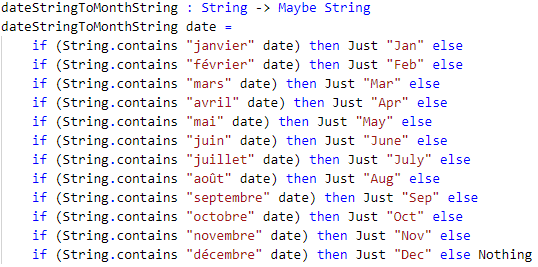
\includegraphics[width=12cm,height=10cm,keepaspectratio]{monthTranslator.PNG}%
\caption{Übersetzerfunktion für Monate im ParallelCoordinates-Modul}
Quelle: Eigene Darstellung
\label{monthTranslator}
\end{center}
\end{figure}

Weiterhin ist noch die Baumvisualisierung zu betrachten, die ebenfalls auf einer View-Funktion aufbaut. Diese erhält als Input einen Record vom Typ GeoTree, was eine eigene Datenstruktur zur Abbildung von Region-Länder-Bäumen unter Verwendung der Dict-Datenstruktur ist, und einen Record vom Typ Filter. Die Übersetzung des GeoTree in eine TreeDiagram.Tree-Datenstruktur übernimmt die ausgelagerte buildTree-Funktion (siehe Abbildung \ref{buildTree}). Diese Funktion bekommt als Input einen GeoTree mit den zu zeichnenden Regionen als Liste von Strings und den zu zeichnenden Ländern als Dictionary mit der jeweils übergeordneten Region als Key und einer Liste von untergeordneten Ländern als Value.\\ Zuerst wandelt buildTree das Länder-Dictionary um in ein Dictionary mit Regionen als Key und Listen von Tree.node als Value. Hierfür werden die Länder jedes Region-Länder-Paares einzeln betrachtet. Diese einzelnen Länder werden anschließend jeweils in die Tree.node Datenstruktur umgewandelt. Hierbei erhält jeder Knoten seinen Ländernamen als Wert und eine leere Liste als Kindknoten, um diese als Blätter zu kennzeichnen. Im nächsten Schritt werden nach ähnlichem Prinzip die Regionsknoten der darüber liegenden Baumebene zusammengestellt. Das Country-Node-Dictionary wird nach jeder Region der Regionenliste durchsucht und zusammen mit den gefundenen Länderknoten als Kindknoten und dem Namen der Region als Wert mithilfe einer map-Funktion in eine Regionknotenliste umgewandelt. Im letzten Schritt wird diese fertige Liste von Teilbäumen in einer gemeinsamen Wurzel mit dem Wert \glqq Afrika\grqq{} zusammengeführt.\\ Der Filter-Record der View-Funktion enthält eine Liste aller aktuell aktiven Regionen und Länder. Diese werden an jeden Aufruf der Funktion \glqq drawnode\grqq{} weitergegeben, welche für das Zeichen einzelner Knoten zuständig ist. Hier wird überprüft, ob der Wert des Knotens mit einem der Werte des Filters übereinstimmt. Ist dies der Fall, so wird für diesen Knoten eine CSS-Klasse \glqq activeNodeBox\grqq{} verwendet, mit welcher der Knoten grün ausgefüllt wird.\\

\begin{figure}[]
\begin{center}
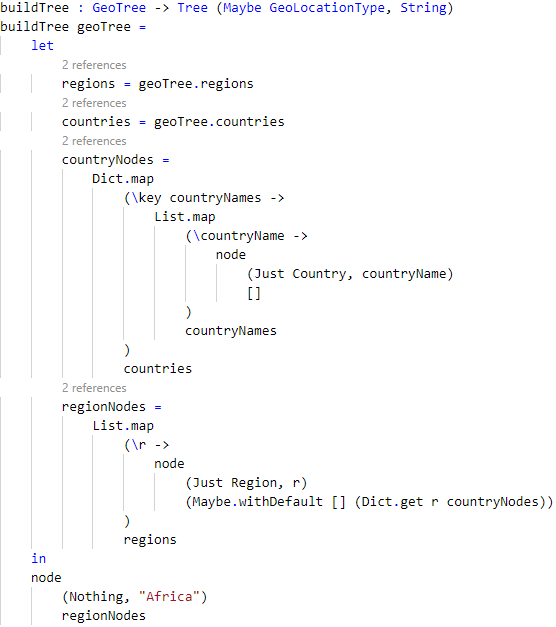
\includegraphics[width=12cm,height=12cm,keepaspectratio]{buildTree.PNG}%
\caption{Funktion für den Bau einer Tree-Datenstruktur im Tree-Modul}
Quelle: Eigene Darstellung
\label{buildTree}
\end{center}
\end{figure}

Interaktive Elemente der Anwendung wurden mithilfe von Elm-Html.Event-Funktionen und CSS umgesetzt. Die klickbaren Rechtecke des Scatterplots, welche durch Maus-Hover angezeigt werden, werden beispielsweise mithilfe konstanter Pixelwerte zusammengestellt und anschließend mit einer Skalierungsfunktion und der zugehörigen Jahreszahl an den korrekten X-Achsenabschnitt verschoben (siehe Abbildung \ref{yearSelectionBox}). Durch einen Klick auf ein solches Rechteck wird eine Html.Events.onClick-Funktion ausgelöst, wodurch die Hauptansicht auf die zweite Visualisierung, unter Mitnahme der Jahreszahl dieses Abschnittes, umgeschaltet wird. Der Hover-Effekt solcher Boxen wurde mithilfe der CSS-Hover-Funktion in der Klasse \glqq yearSelection\grqq{} umgesetzt.\\ Die zweite Visualisierung bietet insgesamt drei Bulma-Buttons als Interaktionsmöglichkeiten. Der \glqq Back\grqq-Button schaltet die Hauptansicht zurück auf die erste Visualisierung. Die verbleibenden beiden Buttons können für das erhöhen oder verringern der aktuell dargestellten Jahreszahl verwendet werden. Hierfür wird durch einen Klick auf den jeweiligen Button erneut ein Ansichtswechsel auf die zweite Visualisierung befohlen. Dabei wird jedoch die aktuelle Jahreszahl um den Wert 1 erhöht oder verringert übergeben, um den gewünschten Effekt zu erzielen.\\ Für die letzte Interaktionsmöglichkeit der Anwendung, die klickbaren Knoten des Filterbaumes, wurde im Stýlesheet eine eigene Hover-Animation erstellt, da für die Knoten keine fertigen Bulma- oder Html-Buttons verwendet wurden. Der Klick auf einen Knoten löst auch hier wieder eine Html.Events.onClick-Funktion aus, wodurch wiederum ein Update des aktuellen Filters im Model verursacht wird.\\

\begin{figure}[]
\begin{center}
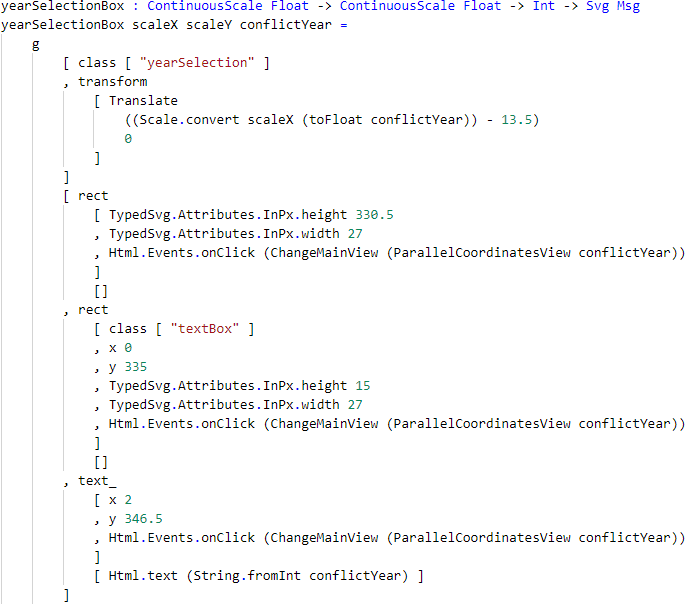
\includegraphics[width=12cm,height=12cm,keepaspectratio]{yearSelectionBox.PNG}%
\caption{Svg-Funktion für eine Box zur Jahresauswahl im Scatterplot-Modul}
Quelle: Eigene Darstellung
\label{yearSelectionBox}
\end{center}
\end{figure}

\section{Anwendungsfälle}

\subsection{Anwendung Visualisierung Eins}
Bei der alleinigen Betrachtung von Ghana, Westafrika im Scatterplot von 2012 bis 2020 fällt auf, dass die Datenpunkte des untersten Bereiches wesentlich dunkler ausfallen als alle anderen. Hieraus ist auf eine hohe Konfliktdichte im Vergleich zu den Vorjahren zu schließen. Durch diese Information sind die Zielgruppen gewarnt, dass aktuell ein erhöhtes Konfliktpotenzial in Ghana besteht, dabei jedoch nur von wenigen Todesopfern auszugehen ist. Hierdurch könnten Hilfseinsätze entsprechend vorbereitet werden oder auch das Land für eine potenzielle Reisewarnung erfasst werden. Die genannte Information hätte auch mithilfe einer Zeitreihe zur Konfliktanzahl pro Jahr gefunden werden können. Diese Möglichkeit wäre in diesem Fall effektiver, da auf diese Weise die genaue Anzahl der Konflikte abgelesen werden könnte und so ein eventueller Abfall oder ein Anstieg der Konfliktzahlen verzeichnet werden könnte.\\

\subsection{Anwendung Visualisierung Zwei}
Stellt der Nutzer den Filter auf Ghana, Westafrika ein und wählt im Scatterplot das Jahr 2017 aus, so werden diesem parallele Koordinaten präsentiert. Hier ist abzulesen, dass sich sämtliche Konflikte dieses Jahres auf das gesamte Jahr recht gleichmäßig verteilen. Auf der mittleren Achse verdichten sich die Konfliktpfade im unteren Teil, wodurch klar wird, dass in den allermeisten Fällen weniger als fünf Menschen in den Konflikten 2017 ums Leben kamen. Zuletzt zeigt die rechte Achse, welche Konfliktarten besonders häufig auftraten. In diesem Fall waren es Aufstände, Schlachten und gewalttätige Handlungen gegen Zivilisten. Die Zielgruppen müssen sich also auf eine Zeit mitten in einem größeren Konflikt, können von weiteren Todesopfern ausgehen und wissen mit welcher Art von Konflikten sie größtenteils zu rechnen haben bei der Vorbereitung von Hilfseinsätzen und der Erstellung von Reisewarnungen.\\ Die genannten Informationen könnten vielleicht besser mithilfe von Sternkoordinaten visualisiert werden, da auf diese Weise Cluster besser sichtbar werden könnten. Für diese Art der Visualisierung wurden jedoch sehr wenige Achsen ausgewählt, um die Vorzüge dessen sinnvoll zu nutzen. Weiterhin benötigt der Umgang mit Sternkoordinaten einen gewissen Grad an Übung und bringt für unsere Anwendung für Laien, die lediglich einen einfachen Überblick gewinnen wollen, zu viel Einarbeitungsaufwand.\\

\subsection{Anwendung Visualisierung Drei}
Mithilfe des Filterbaumes können einfache Erkenntnisse über geografische Zusammenhänge innerhalb Afrikas während der Benutzung der Anwendung gewonnen werden. Entdeckt beispielsweise ein Nutzer, dass Ghana seit 2012 von vielen Konflikten betroffen ist, so könnte dieser Länder aus der gleichen Region auf ähnliche Informationen untersuchen wollen. Hier ermöglicht es der ausklappbare Filterbaum einen klaren Überblick über die Regionen Afrikas zu behalten, indem uninteressante Länder verdeckt und interessante Länder hierarchisch nach Regionen geordnet werden. So könnte ein Mitarbeiter des auswärtigen Amtes ohne die Nutzung einer zweiten Quelle sehr effizient weitere potenziell betroffene Länder für eine Reisewarnungsuntersuchung ausmachen.\\ Eine alternative Möglichkeit zur Darstellung der hierarchischen Zusammenhänge Afrikas wäre die Visualisierung der Regionen und Länder als impliziter Baum. Diese Möglichkeit ist jedoch wesentlich weniger für die interaktiven Filterfunktionen geeignet, welche der Baum gleichzeitig bieten soll. Die Button-Größen würden hier zu stark variieren und die Schachtelung der Teilbäume würde nur Blätter (also Länder) des Baumes als Buttons zulassen.\\

\section{Verwandte Arbeiten}
Eine themenverwandte Arbeit aus dem Jahr 2013 trägt den Titel \glqq VISUALIZATION OF MULTIDIMENSIONAL DATA IN PURPOSE OF QUALITATIVE CLASSIFICATION OF VARIOUS TYPES OF COAL\grqq{} \cite{coal}. Hier wird die vorher kaum wahrgenommene Möglichkeit besprochen, Eigenschaften verschiedene Kohletypen multidimensional zu visualisieren, um diese im Vergleich zu analysieren. Vor allem Abbildung 7 der Arbeit ist besonders interessant für dieses Projekt. Diese Abbildung zeigt eine Datenmenge in sieben Dimensionen visualisiert als parallele Koordinaten.\\ Gemeinsamkeiten dieser Visualisierung mit den parallelen Koordinaten unserer Anwendung bestehen in der klassischen Umsetzung mit parallelen, senkrechten Achsen und den Pfaden über diesen, welche je ein Datenobjekt repräsentieren. Die Unterschiede hingegen liegen in der höheren Achsenanzahl, fehlender Achsenbeschriftungen und der Verwendung von drei verschiedenen Helligkeitsstufen der Pfade für unterschiedliche Datenobjekte (in diesem Fall Kohlearten).\\ Ein solcher Ansatz könnte durchaus auch interessant für unsere Anwendung sein. Es könnte beispielsweise dabei helfen verschiedene Länder und Regionen zu unterscheiden, womit die jetzige Visualisierung noch Probleme hat. Da jedoch potenziell 18 unterschiedliche Länder angezeigt werden könnten in den parallelen Koordinaten wird schnell klar, dass hier nicht nur mit Helligkeitsstufen gearbeitet werden kann. Eine bessere Variante wäre die Darstellung der fünf Regionen als klar unterscheidbare Farben. Innerhalb dieser Regionen könnten Länder dann in Helligkeitsstufen eingeteilt werden.\\

Eine weitere themenverwandte Arbeit ist \glqq Designing and Implementing an Interactive Scatterplot Visualization for a Tablet Computer\grqq{} \cite{tablet}. Diese Arbeit zielt darauf ab, mögliche Designs für interaktive Informationsvisualisierung auf Tablets zu erforschen und zu diskutieren, um die Möglichkeiten dieser Geräte in Zukunft besser ausschöpfen zu können. Im Rahmen dieser Arbeit wurde eine Anwendung entwickelt, welche neuartige Interaktionsmöglichkeiten mit Scatterplots auf dem Tablet umsetzt. Unter anderem wird hierbei die Selektion von Datenpunkten behandelt, welche ebenfalls im Scatterplot unserer Anwendung eine Rolle spielt.\\ Speziell für diesen Aspekt wurden in der Arbeit in Kapitel 5.1 ähnliche aber auch abweichende Konzepte vorgeschlagen, wie sie bereits auf ähnliche Weise in unserer Anwendung verwendet wurden. Eine dieser ähnlichen Techniken ist der \glqq Off-centered pointer\grqq. Hier tippt und hält der Nutzer seinen Finger auf den Bildschirm, um einen Mauszeiger erscheinen zu lassen, mit einer leicht versetzten Position zum Berührungspunkt. Dieser Mauszeiger kann nun durch Verschiebung des Berührungspunktes bewegt werden und Hover-Effekte auslösen. Durch Anheben des Fingers wird eine Selektion, ähnlich einem Mausklick, ausgelöst. Diese Variante stellt lediglich eine Art Desktop-PC-Port für Tablets dar und könnte genau so für unsere Anwendung auf dem Tablet verwendet werden.\\ Eine zweite Variante eines ähnlichen Scatterplot-Interaktionsdesigns ist das \glqq Axis pan\grqq. Hierbei hält der Nutzer einen Punkt der Achse gedrückt und kann diesen Punkt auf der Achse verschieben, um eine ganze Zeile oder Spalte des Scatterplots mit einer vertikalen oder horizontalen Referenzlinie zu markieren. Durch Anheben des Fingers wird dann die markierte Datenpunktmenge selektiert. Diese Variante ähnelt unserer Anwendung durch die Umsetzung einer Spaltenauswahl. Diese ist aber natürlich im Vergleich zu unserer Umsetzung nur auf dem Tablet anstatt dem Desktop-PC anwendbar. Eine der beiden genannten Varianten könnte sich durchaus als hilfreich für eine Tablet-Umsetzung des Programms unserer Arbeit herausstellen.\\

\section{Zusammenfassung und Ausblick}
Im Rahmen dieses Projektes entstand eine Anwendung, welche es einem Nutzer ermöglicht sich einen Gesamtüberblick über die Konflikte Afrikas von 1997 bis 2021 in Hinsicht auf Zeitpunkt, Todeszahlen und Konfliktart mit geografischem Bezug zu verschaffen. Hierbei wurde der zur Verfügung stehende Datensatz nicht in vollen Zügen ausgeschöpft, was zukünftigen Versionen der Anwendung noch weiteren Raum zur Erweiterung bietet. Andererseits werden jedoch bei der Visualisierung des Datensatzes auch keine, für die Zielgruppen essenziell wichtigen Aspekte vernachlässigt.\\ Mithilfe der entstandenen Anwendung können Hilfsorganisationen einen Überblick bewahren, an welchen Orten Afrikas Hilfseinsätze infrage kommen könnten. Weiterhin kann es mithilfe des Programms Mitarbeitern des Auswärtigen Amtes leichter fallen, einen Überblick zu erhalten, welche Länder Afrikas dringend einer genaueren Gefahreneinschätzung unterzogen werden müssen, um Reisende ausreichend zu warnen. Hierbei fällt die eigentliche Anwendung jedoch noch recht unpräzise aus und vernachlässigt wichtige Aspekte, welche nicht durch den verwendeten Datensatz vermittelt werden. Aus diesem Grund sollten zur Erfüllung von den genannten kritischen Aufgaben dringend neben der Anwendung weitere Informationsquellen herangezogen werden. Die Anwendung selbst sollte als ein Werkzeug betrachtet werden, um die Aufmerksamkeit der Zielgruppe auf Regionen von Interesse zu lenken.\\

Aus den Untersuchungen dieser Arbeit geht hervor, dass die Kombination einer Scatterplot-Visualisierung und der X-Ray-Technik für die angedachte Aufgabe nicht präzise genug ist. Es sind durchaus hohe und niedrige Konfliktdichten erkennbar, diese lassen sich jedoch kaum unterscheiden geschweige denn die Annahme eines Trends zu. In zukünftigen Arbeiten wäre hier das Ersetzen des Scatterplots durch eine Zeitreihe über die Konfliktdichten pro Jahr sinnvoller, da auf diese Weise An- und Abstiege besser zu erkennen sind. Die Todeszahlen können ohnehin in den parallelen Koordinaten abgelesen werden.\\

Eine weitere Anpassung könnte in den parallelen Koordinaten erfolgen. Hier ergibt sich das Problem, dass bei einer zunehmenden Anzahl an Datenobjekten ein genaues Ablesen der Darstellung immer schwerer gestaltet. Eine Unterscheidung von Regionen durch Farben und einzelner Länder durch Helligkeitsstufen könnte Nutzern von zukünftigen Versionen der Anwendung einen klaren Vorteil bei der geografischen Unterscheidung von Konflikten verschaffen. Das Ableseproblem bei einer hohen Konfliktdichte könnte bei der Umsetzung dieser Variante jedoch auch bei einzelnen, besonders betroffenen Ländern auftreten, da hier erneut alle Datenobjekte ununterscheidbar sind. In diesem Fall könnte eventuell die Anwendung der X-Ray-Technik Abhilfe schaffen.\\

Zuletzt ist noch das Auslassen der Koordinaten-Daten des Datensatzes zu den Konflikten als Ausblick anzumerken. Durch Ergänzung von Länder-Polygonzügen könnte hiermit eine Karte mit den Konfliktorten als vierte Visualisierung in die Anwendung eingebaut werden. Dabei ist sogar eine Verwendung von Selektionstechniken denkbar, um den Filterbaum zu ersetzen und weiterer Visualisierungsfläche Platz zu schaffen. Nichtsdestotrotz würde eine solche Karte dem Nutzer ein sehr genaues Bild der geografischen Zusammenhänge mit den Konflikten vermitteln und eine sinnvolle Ergänzung der Anwendung darstellen.\\

\section*{Anhang: Git-Historie}
\begin{verbatim}
* 4ff7ba5 (HEAD -> main, origin/main, origin/HEAD)
          (Bericht: Rechtschreibkorrektur, 2021-09-11)
* 1dbf4a5 (Bericht: bibliography, 2021-09-11)
* f8f63c9 (Bericht: Zuammenfassung, 2021-09-11)
* 6b6bfcc (Bericht: Anwendungsfälle, 2021-09-10)
* cffb61d (Bericht: Implementierung, 2021-09-10)
* 5bf99a8 (Bericht: Interaktion, 2021-09-09)
* c44327a (implementation notes, 2021-09-08)
* 17a9cf5 (imports sorted, 2021-09-08)
* 925fc08 (Bericht: Visualisierung 2 & 3, 2021-08-31)
* fdc33e3 (Bericht: Visualisierung 1, 2021-08-30)
* 4906244 (Bericht: Präsentation der Visualisierungen, 2021-08-29)
* 480b33c (Bericht: Anforderungen an die Visualisierungen, 2021-08-29)
* feb8b0f (Bericht: Analyse der Anwendungsaufgaben, 2021-08-29)
* b588c3a (Bericht: Datenvorverarbeitung, 2021-08-28)
* 28c9d27 (Bericht: Daten, 2021-08-28)
* 7fb0a27 (Bericht: Überblick & Beträge + Stichpunkte, 2021-08-26)
* 1145714 (cleanup conflict type, 2021-08-26)
* 865bfe3 (Bericht: Zielgruppe, 2021-08-26)
* d735fdb (Bericht: Anwendungshintergrund, 2021-08-26)
* a2fc9f1 (Bericht: Einleitung, 2021-08-25)
* 871c73f (cleanup, 2021-08-25)
* 42af250 (url change, 2021-08-24)
* 784898c (cleanup, 2021-08-24)
* 0798251 (show names on hover, 2021-08-24)
* bea8f0e (remove old filter, 2021-08-24)
* 404f0d8 (remove locations (too many for tree), 2021-08-24)
* 06a9346 (main title, 2021-08-23)
* 1b1081c (better filter + cleanup, 2021-08-23)
* e57db4b (styling, 2021-08-23)
* f4e71e6 (empty filter fix, 2021-08-23)
* e2b0175 (node styling, 2021-08-23)
* 01105d4 (styling, 2021-08-23)
* 11501a0 (css stylesheet, 2021-08-23)
* abfe117 (choosing filter works, 2021-08-23)
* fb14de9 (filter update functions, 2021-08-23)
* 284d208 (breadcrumbs correct disabled, 2021-08-23)
* acfd4e1 (rotation of nodes changed, 2021-08-23)
* 0380df3 (buildTree finished, 2021-08-23)
* f256415 (use Dicts for GeoTree, 2021-08-23)
* 633961f (use dicts for GeoTree, 2021-08-23)
* 72c951a (data preprocessing for rendering tree, 2021-08-23)
* 943a3d2 (getTreeData + renaming, 2021-08-23)
* 47a37c5 (filter type and filter update, 2021-08-23)
* 189e61d (renaming, 2021-08-23)
* b95aa00 (geo filter navigation, 2021-08-23)
* 8b7c067 (import Tree, 2021-08-23)
* 1fd9edb (tree: renderTree, 2021-08-23)
* 7c2b7a0 (tree: buildTree, 2021-08-23)
* 1928d0f (tree: drawnode, 2021-08-23)
* c4ec1ad (tree: drawline, 2021-08-23)
* 31bc74b (algeria as init country, 2021-08-22)
* 59a1354 (title, 2021-08-22)
* fd4b60d (year switch buttons, 2021-08-22)
* 6053d80 (pc scaling fix, 2021-08-22)
* d6005b3 (scatterplot scales adaptive, 2021-08-22)
* c318255 (filter for correct year selection, 2021-08-22)
* 73aec08 (back button, 2021-08-22)
* 35337fa (refactoring, 2021-08-22)
* 54ae3b2 (view change possible, 2021-08-22)
* 477d79e (field name change from model updated, 2021-08-22)
* 240518a (model updated, 2021-08-22)
* 7109bac (import pc, 2021-08-22)
* 561008d (conflicts updated, 2021-08-22)
* 128a86f (pc: mapping functions, 2021-08-22)
* 9b17e9a (pc: declare axes, 2021-08-22)
* a3f2541 (pc: map conflicts to desired values, 2021-08-22)
* 6925569 (pc: y scale local, 2021-08-22)
* 685ba51 (pc: draw segments, 2021-08-22)
* 0152b39 (pc: render parallel coordinates, 2021-08-22)
* d1f2c29 (pc: y axis ordinal, 2021-08-22)
* e7357f3 (pc: y axis, 2021-08-22)
* 468f73d (pc: imports, 2021-08-22)
* c59822c (pc: constants, 2021-08-22)
* bf3fc58 (refactoring to create multi page app, 2021-08-20)
* 6561545 (introduce viewTypes, 2021-08-20)
* 7f4988f (render year selection boxes, 2021-08-20)
* 66436d8 (css class changes, 2021-08-20)
* ab1347b (refactoring, 2021-08-20)
* 4f73ecd (fix: country checkboxes, 2021-08-20)
* 523f9dd (filter for Countries works + keep axes scalings, 2021-08-20)
* f2dd513 (render scatterplot country checkboxes, 2021-08-18)
* a2b6e83 (render scatterplot country list, 2021-08-18)
* c583eab (update scatterplot country list, 2021-08-18)
* 4c977e2 (view refactoring, 2021-08-18)
* 0dea1e9 (bulma styling, 2021-08-18)
* 978d843 (main.js updated, 2021-08-18)
* 0fc19d5 (init Tree.elm, 2021-08-18)
* f2e9e0b (init ParallelCoordinates.elm, 2021-08-18)
* cece348 (render Scatterplot, 2021-08-18)
* 4d99eaf (import Scatterplot, 2021-08-18)
* b11b66d (scatterplot view function, 2021-08-18)
* a7fe5ae (scatterplot render function, 2021-08-18)
* f6d71ab (point render function, 2021-08-18)
* 41d4f04 (axis functions, 2021-08-18)
* ecf419c (scale functions, 2021-08-18)
* 34987a2 (init constants, 2021-08-18)
* 8f4c4d8 (init Scatterplot, 2021-08-18)
* a77404e (load conflicts data, 2021-08-18)
* 06afe1b (conflict json decoder, 2021-08-18)
* 2fa48e6 (conflict type, 2021-08-18)
* 89c886a (init Conflict.elm, 2021-08-18)
* a03226b (init bulma, 2021-08-18)
* bdded9a (init json data, 2021-08-18)
* 7e3dd82 (report init, 2021-07-17)
* f7226b9 (readme fix, 2021-07-17)
* 838b79b (project init, 2021-07-17)
* 35f9999 (Initial commit, 2021-07-17)
\end{verbatim}
\printbibliography

\end{document}

